\section{ANALYSIS AND PRELIMINARY RESULTS}

In order to study the socio-technical congruence hypothesis for the Cargo package manager, I started analysing its package dependency network and the associated technical and social (commenting) activities of its GitHub contributors.
To do so, I focused on the three preliminary research questions presented in Section~\ref{sec:intro}.

%TOM:Commented out, I do not think you need this any longer...
%Intutively according to Conway's law \cite{Conway1968} we guess if there is some technical dependency between software packages, it will be more likely that there is also a collaboration between package contributors (through commits, pull requests, and their associated comments).

%TOM: Only introduce the terminology that you really need. (Since you have only 2 pages to explain things, I do not know if you will need a lot of terminology to explain...
%We introduce the following terminology to talk about how packages and contributors linked to each other in a social or technical network. We use the term 'Dependency' Where a software component uses another package inside it and 'Reverse dependency' where a package is used as a required package in another software component.

{\color{red}@MEHDI: First repeat the RQ presented in Section~\ref{sec:intro}, then explain what was the intuition behind the question, and how you will "operationalise" and find evidence for this RQ in the specific Cargo case study, and then explain which initial evidence (if any) you have found.}
  
  
\textbf{RQ1 - }According to our findings there are less comment on packages with technical dependency than others but comments on packages which are dependent to each other are increasing as we move toward 2019. It seems that this tendency is going to grow more in recent years. Our investigation shows, the peak in Febraury 2016 caused by a major problem with 2 popular component which was led to a burst of comment by both users and contributors of those packages.

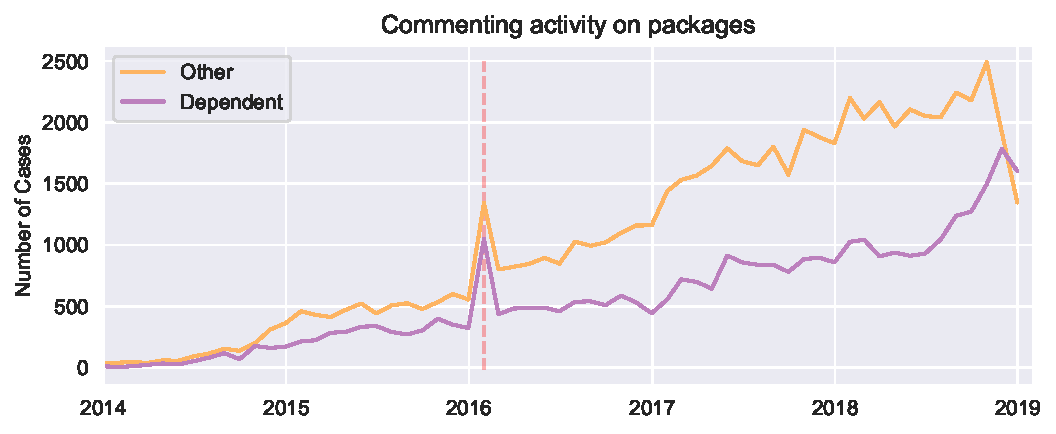
\includegraphics[width=\columnwidth]{Photos/RQ1_1.pdf} 